\section{Extended Analysis}
\label{app:extended}

While the results in Section~\ref{sec:comparison} are good,
it is desirable to have a more extensive analysis.
The only algorithms tested are
\UnrolledThree{} (Listing~\ref{list:newton-unrolled-3}),
\WhileOne{} (Listing~\ref{list:newton-while-1}),
\WhileTwo{} (Listing~\ref{list:newton-while-2}), and
\WhileThree{} (Listing~\ref{list:newton-while-3}),
as these performed the best.
The deterministic and random values will be separated.
All values tested in Section~\ref{sec:comparison}
are included in these tests.

\subsection{Deterministic Tests}
\label{app:deterministic}

\subsubsection{Overview}

We test additional deterministic values.
First, we include all deterministic values from Section~\ref{sec:comparison}.
Additional values are of the form $2^{k} + 2^{j}$ for $j,k\in\N$ and $j < k$.
The total number of values were 33154.
The results are shown in Table~\ref{table:minimal_gas_costs_ed}
and Figure~\ref{fig:minimal_gas_hist_ed}.

The minimal values have a somewhat different trend than before:
\UnrolledThree{} still performs well for larger numbers,
but \WhileOne{} does very good, too.
This may be explained by the initialization value in this instance
starting \emph{very close} to the actual value;
see the discussion in Appendix~\ref{app:deterministic_detailed}.
It is interesting that \UnrolledThree{} performed as well as it did
in this situation which favors \WhileOne{}.

The results here show that it is easy to (unwittingly)
test values which are biased toward one particular algorithm.
This is the reason for testing a large collection
of random values in Appendix~\ref{app:loguniform}.

\subsubsection{Detailed Look}
\label{app:deterministic_detailed}

We now take a closer look at particular values:
we look at all values $2^{254} \le v < 2^{255}$
and then $2^{255} \le v < 2^{256}$.
In this instance, we are just comparing the gas cost of \UnrolledThree{}
and \WhileOne{}.
We expect these two collections to be characteristic
of the remaining gas values.

\paragraph{Values $2^{254} \le v < 2^{255}$}
For \UnrolledThree{}, there are only two gas costs in this range:
$824$ and $831$.
\WhileOne{} starts off at a low gas cost of $616$;
it then jumps to $706$, $796$, $886$, $976$, and $1066$.
We estimate that each Newton iteration costs $90$ gas.

\paragraph{Values $2^{255} \le v < 2^{256}$}
For \UnrolledThree{}, the gas cost is predominantly $824$;
there is one instance of $831$, and three values of $168$ (from early exit).
Almost all gas cost values for \WhileOne{} are $1066$,
with some larger values and a few smaller (early exit).

\begin{table}[p]
\centering
\begin{tabular}{|c|S[table-format=5.0]|}
\hline
Total & 33154 \\
\hline
\cellcolor{yellow!25} \UnrolledThree{} & \cellcolor{yellow!25} 15769 \\
\cellcolor{yellow!15} \WhileOne{}      & \cellcolor{yellow!15} 15639 \\
\WhileTwo{}      &   133 \\
\WhileThree{}    &  1628 \\
\hline
\end{tabular}
\caption[Minimal Gas Costs Statistics]{Here are number of times
    each method had minimal gas costs;
    these are results for the additional deterministic values
    based around powers-of-2.
    These results are for the tests in Appendix~\ref{app:deterministic}.
    }
\label{table:minimal_gas_costs_ed}
\end{table}

\begin{figure}[p]
\centering
    \begin{subfigure}[t]{0.45\textwidth}
    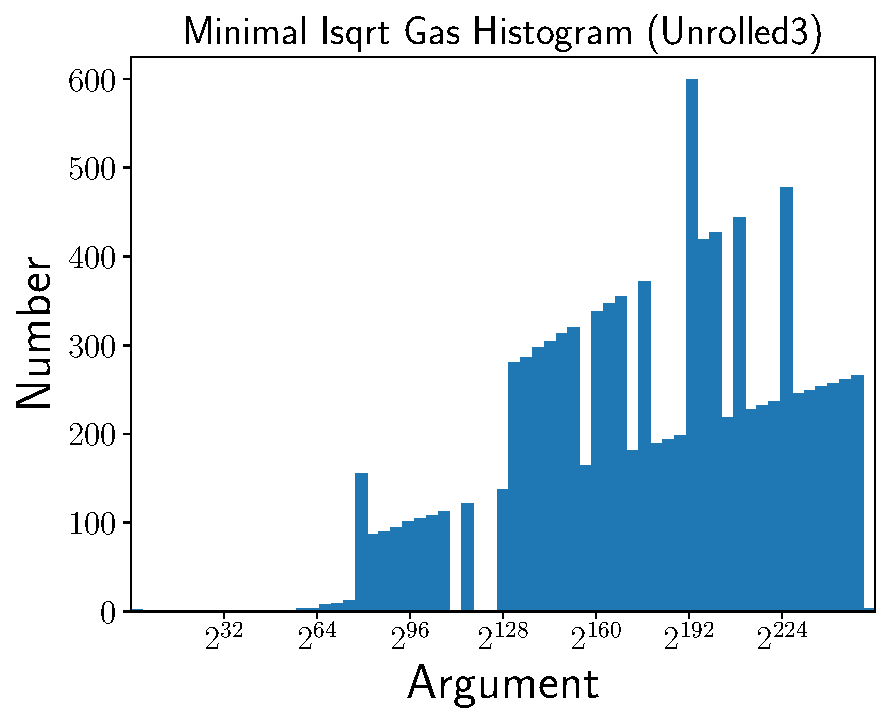
\includegraphics[width=\textwidth]{plots/minimal_hist_Unrolled3_ed.pdf}
    \end{subfigure}
    \begin{subfigure}[t]{0.45\textwidth}
    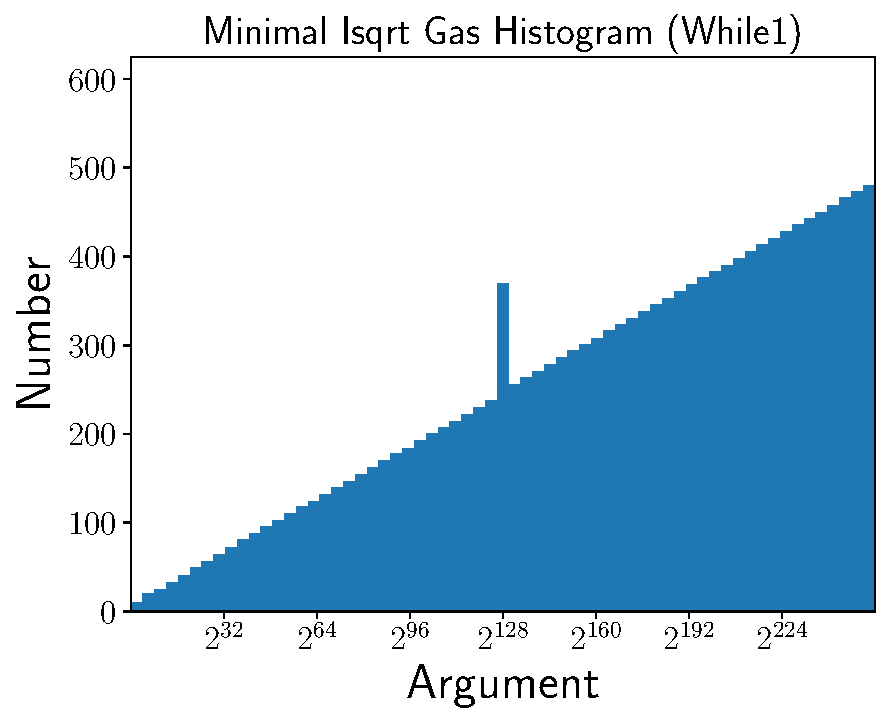
\includegraphics[width=\textwidth]{plots/minimal_hist_While1_ed.pdf}
    \end{subfigure}

    \begin{subfigure}[t]{0.45\textwidth}
    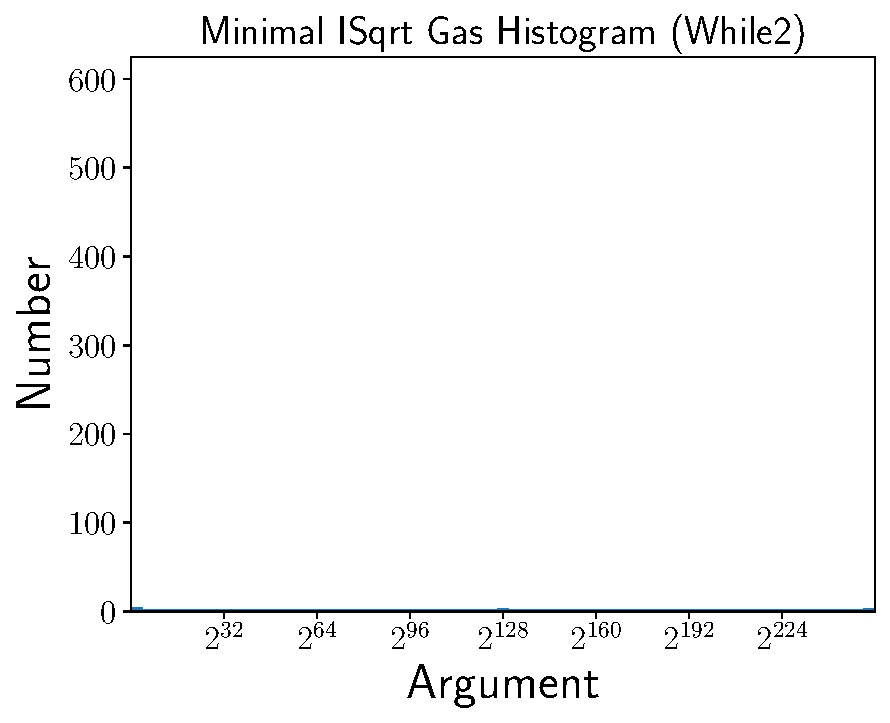
\includegraphics[width=\textwidth]{plots/minimal_hist_While2_ed.pdf}
    \end{subfigure}
    \begin{subfigure}[t]{0.45\textwidth}
    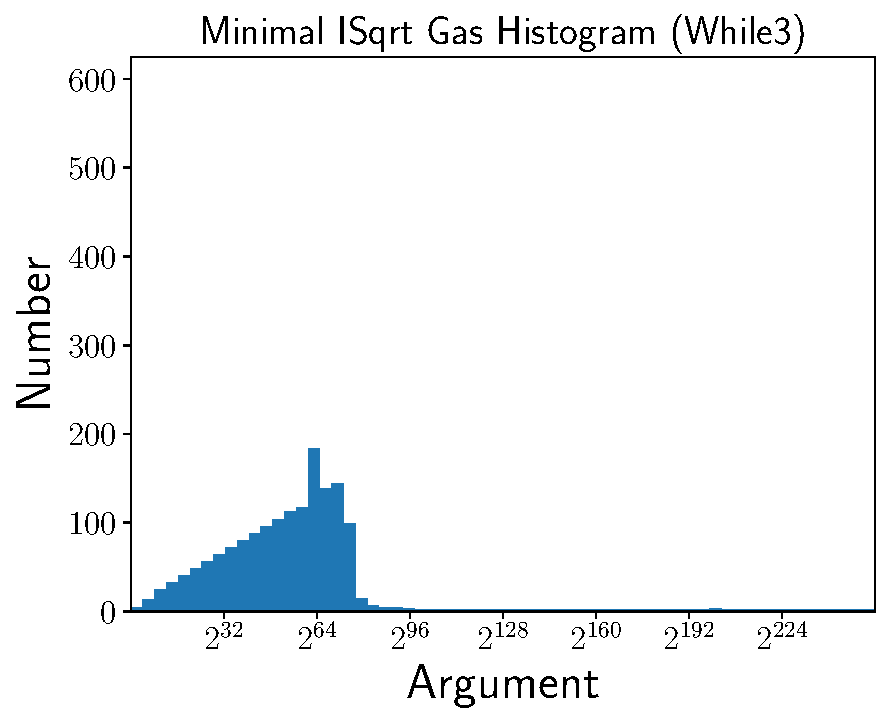
\includegraphics[width=\textwidth]{plots/minimal_hist_While3_ed.pdf}
    \end{subfigure}
    \caption{Here we plot a histogram showing where each algorithm is minimal
        when using a larger sample of deterministic values.
        Each bin counts the total number instances where the algorithm's
        gas cost was minimal.
        These results are for the tests in Appendix~\ref{app:deterministic}.
        }
    \label{fig:minimal_gas_hist_ed}
\end{figure}


\subsection{Loguniform Tests}
\label{app:loguniform}

The tests in Section~\ref{sec:comparison} ran 1280 values
which came from a loguniform distribution~\cite{ScipyLoguniform}.
Here, we perform the same test using more samples;
in particular, we use $16384 = 2^{14}$ random values from 16808 samples.
The results are shown in Table~\ref{table:minimal_gas_costs_er}
and Figure~\ref{fig:minimal_gas_hist_er}.

There is no significant difference between the results in 
Tables~\ref{table:minimal_gas_costs} and \ref{table:minimal_gas_costs_er}
or Figures~\ref{fig:minimal_gas_hist} and \ref{fig:minimal_gas_hist_er}.
The results are clear:
\UnrolledThree{} has almost 75\% of the minimal cost for random values.

\begin{table}[p]
\centering
\begin{tabular}{|c|S[table-format=5.0]|}
\hline
Total & 16384 \\
\hline
\cellcolor{yellow!25} \UnrolledThree{} & \cellcolor{yellow!25} 12183 \\
\WhileOne{}      &  1537 \\
\WhileTwo{}      &   320 \\
\WhileThree{}    &  2347 \\
\hline
\end{tabular}
\caption[Minimal Gas Costs Statistics]{Here are number of times
    each method had minimal gas costs;
    these are results for the additional loguniform random values.
    These results are for the tests in Appendix~\ref{app:loguniform}.
    }
\label{table:minimal_gas_costs_er}
\end{table}

\begin{figure}[p]
\centering
    \begin{subfigure}[t]{0.45\textwidth}
    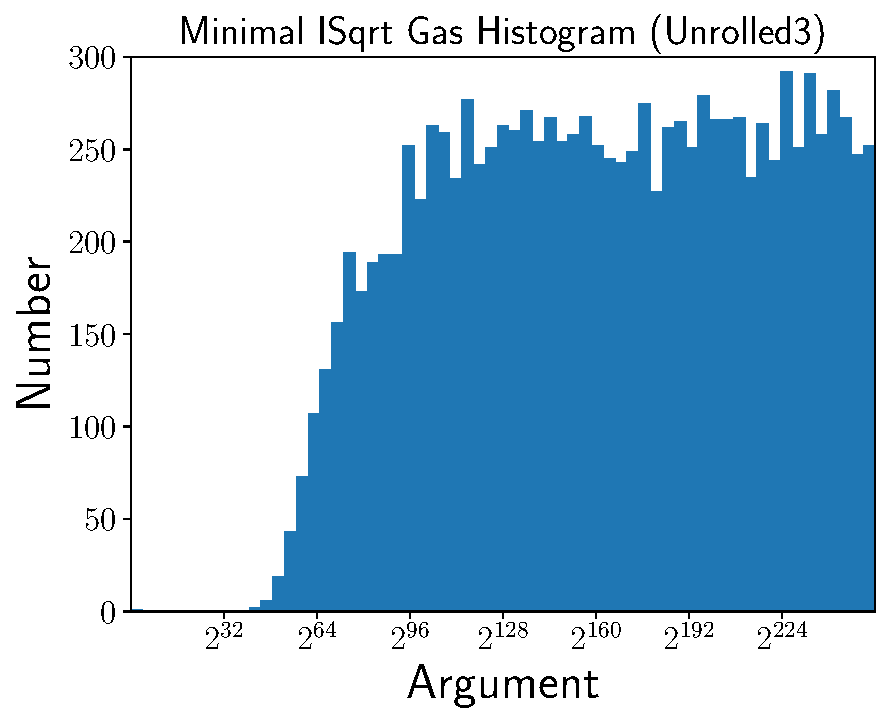
\includegraphics[width=\textwidth]{plots/minimal_hist_Unrolled3_er.pdf}
    \end{subfigure}
    \begin{subfigure}[t]{0.45\textwidth}
    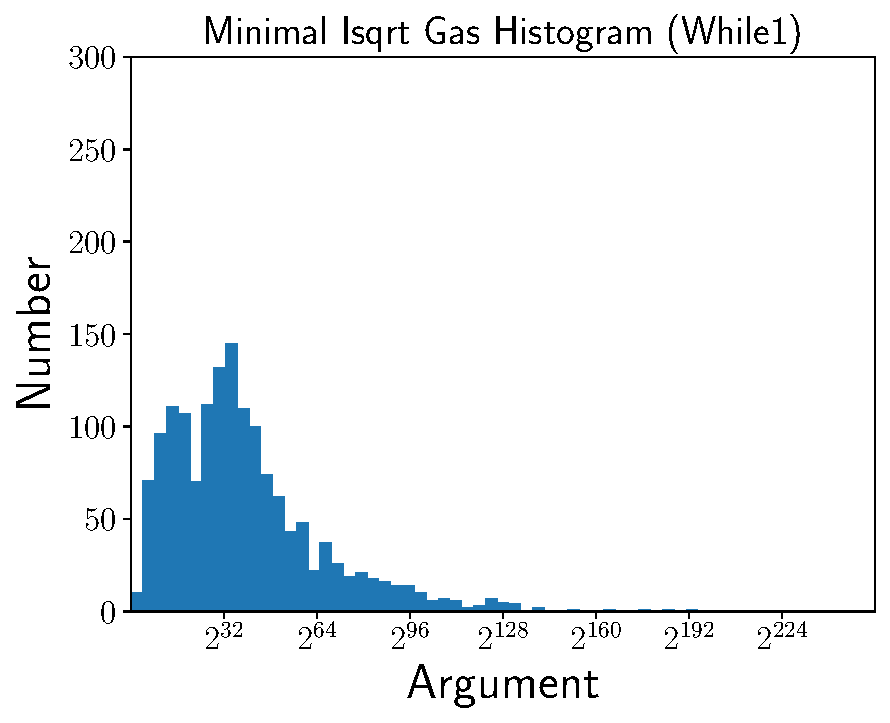
\includegraphics[width=\textwidth]{plots/minimal_hist_While1_er.pdf}
    \end{subfigure}

    \begin{subfigure}[t]{0.45\textwidth}
    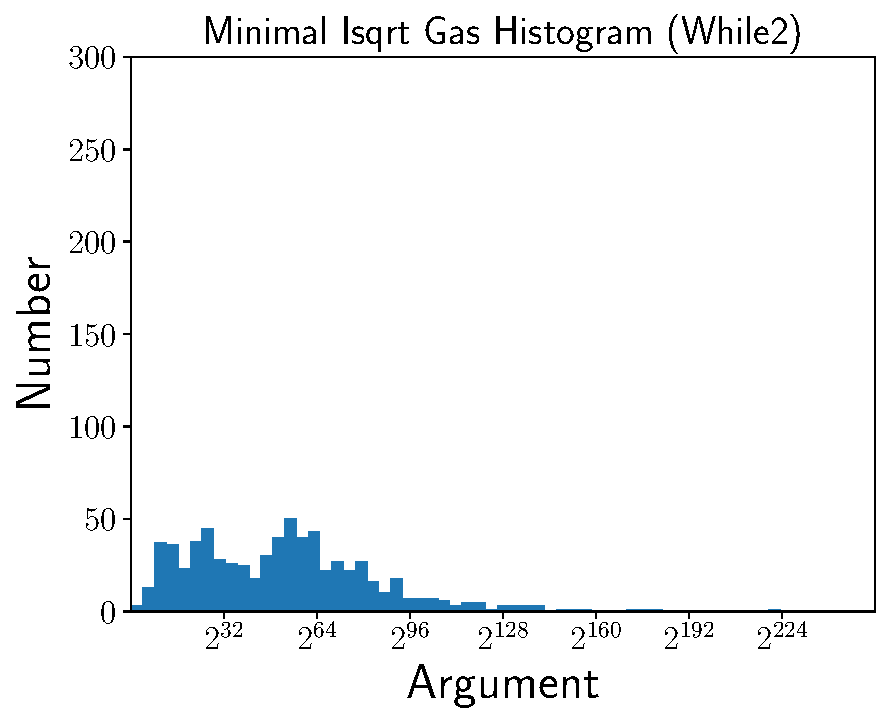
\includegraphics[width=\textwidth]{plots/minimal_hist_While2_er.pdf}
    \end{subfigure}
    \begin{subfigure}[t]{0.45\textwidth}
    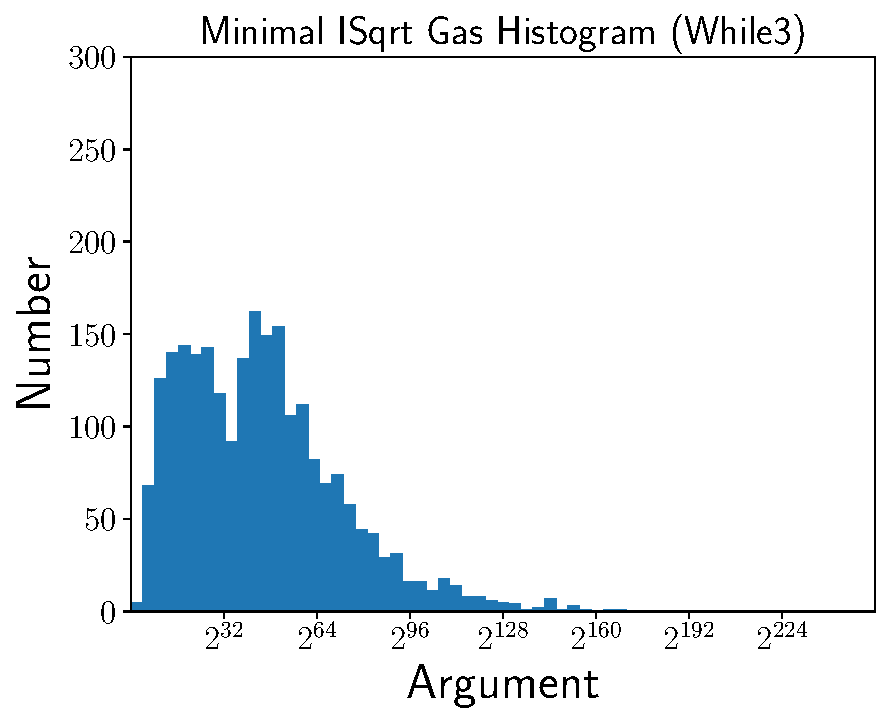
\includegraphics[width=\textwidth]{plots/minimal_hist_While3_er.pdf}
    \end{subfigure}

    \begin{subfigure}[t]{0.45\textwidth}
    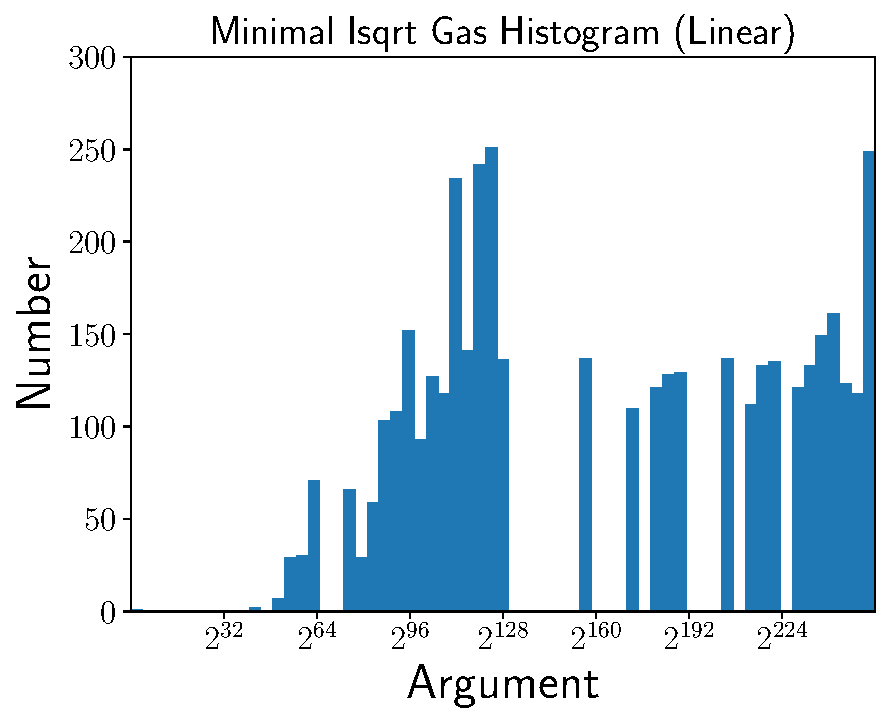
\includegraphics[width=\textwidth]{plots/minimal_hist_Linear_er.pdf}
    \end{subfigure}
    \caption{Here we plot a histogram showing where each algorithm is minimal
        when using a larger sample of loguniform random values.
        Each bin counts the total number instances where the algorithm's
        gas cost was minimal.
        These results are for the tests in Appendix~\ref{app:loguniform}.
        }
    \label{fig:minimal_gas_hist_er}
\end{figure}


\subsection{Conclusion}

This extended analysis gives additional insight into how the algorithms
perform but with the same result:
\UnrolledThree{} is the best algorithm
for a generic \texttt{uint256} value.
